\label{Intro.}
Water has been described as being ``at the centre of the planetary drama of the Anthropocene''
\cite{gleesonIlluminatingwatercycle2020}.
It is essential not only for earth system processes but also in supporting the economic development and continued well-being of human societies. Human activities stemming from our reliance on the water have profoundly modified the natural water cycle, moving rivers dominated by a hybrid of social and natural tendencies
\cite{gleesonIlluminatingwatercycle2020,sivapalanSociohydrologynewscience2012,qinTheoreticalframeworkdualistic2014,abbottwatercycleAnthropocene2019,leviaHomogenizationterrestrialwater2020}.
Facing this major transformation, many big river basins worldwide (which are hot spots of civilization and economic growth) are urgently in need of successful water governance for sustainability
\cite{bestAnthropogenicstressesworld2019,falkenmarkUnderstandingwaterresilience2019,dibaldassarreSociohydrologyScientificChallenges2019}.
As an integral part of a proposed earth system governance framework, water governance requires a deep understanding of changes in the complex relationships between humans and water
\cite{dibaldassarreSociohydrologyScientificChallenges2019,biermannNavigatingAnthropoceneImproving2012,steffenemergenceevolutionEarth2020}.

Governance is essentially about ``who gets what, when and how''. Specifically, water governance refers to the political, social, economic, and administrative systems that influence the use and management of water %! citation.
For water resources in populated areas, missing governance means missing sustainability, and a first important step in understanding transitions toward successful water governance is identifying the different regimes.
\cite{undpwatergovernancefacilityWaterGovernanceIssue}.
Corresponding to ``who gets what, when and how'', the United Nations Development Programme (UNDP) suggests three key dimensions of water use are decided by the water governance directly: ``When and what water to use?'' (supply), ``How water provides different services to well-beings?'' (purpose), and ``Who can use water equally and efficiently?'' (allocation)
\cite{undpwatergovernancefacilityWaterGovernanceIssue, mariajacobsonUserguideassessing2013, kjellenWatergovernanceperspective2015}.
As a locally stable state of a system, function, and dominant controls, habitual relationships between humans and water maintain regimes of water governance
\cite{carpenterEarlyWarningsRegime2011}.
However, large and persistent changes in key properties may lead to a loss of systematical stability, potentially resulting in a regime shift with impacts on system outcomes and widespread cascading effects
\cite{rochaCascadingregimeshifts2018, gregrCascadingsocialecologicalcosts2020}.
Therefore, as both signals and consequences of substantive changes in human-water systems, regime shifts can trigger changes in the three key dimensions of water governance (supply, purpose, and allocation), with new challenges to sustainability %! UNDP year
\cite{undpwatergovernancefacilityWaterGovernanceIssue, mariajacobsonUserguideassessing2013, kjellenWatergovernanceperspective2015}.
First, the supply of water depends not only on climate (with increasing scarcity and uncertainty in many regions) but also on the increasingly insatiable demands from economic activities such as irrigation and industry; water storage can resolve some but not all of these issues
\cite{greveGlobalassessmentwater2018,wadaHumanwaterinterface2017,qinFlexibilityintensityglobal2019}.
Second, the purpose of how water services human well-being is to consider trade-offs between consumptive uses (e.g., drinking and food production) and non-consumptive uses (e.g., energy production)
\cite{liuWaterscarcityassessments2017,florkeWatercompetitioncities2018,kleemannQuantifyinginterregionalflows2020}.
Third, the allocation of water across the whole basin is influenced not only by regionally socio-economic and environmental context but also by systematically regulating resources
\cite{roobavannanRoleSectoralTransformation2017,speedBasinwaterallocation2013}.
Despite regime shifts in water governance related to substantive changes in any of the three dimensions, separately considering their intertwines within human-water systems can lead to holistic failure in governing water.
The lack of a comprehensive but straightforward approach to identifying changes in water governance regimes challenges sustainability, and filling this gap can well align human and water systems (Figure~\ref{fig:framework}).

As an informative example, we focus on the Yellow River Basin (YRB, see \textit{Appendix} Methods S1 and Figure S1 for details), the fifth-largest river in the world.
With drastically anthropogenic intervention, the YRB experienced the most intense water governance challenges in China, leading to long-standing sustainability barriers.
Since the 1960s, the implementation of conservation measures, regulation reservoirs, and levee constructions have contained the issues caused by high-sediment loads
\cite{wangReducedsedimenttransport2016,wuEvolutioneffectssocialecological2020}.
However, water over-use has led to depletions of the over-burdened river, creating new governance challenges that have been addressed through a range of related policies (e.g., regulating water use and limiting water withdrawals)
\cite{xiaDevelopmentWaterAllocation2012}.
Today, it is still impossible to completely cover water demands, balance trade-offs between ecosystem services, and lead to equities in different regions; -who gets water, when and how is still an open question for sustainable water governance
\cite{wangYellowRiverwater2019,wohlfartSocialecologicalchallengesYellow2016}.
The YRB has been among the most rapidly-changing large river basins worldwide, with myriad responses to the endless governance challenges induced by environmental, economic, social and political factors. Identifying regime shifts in water governance within the YRB can thus provide crucial insights into rapidly-changing big river basins and how governance may respond to meeting challenges to their sustainability.

% 这里我们整合了三个方向,提出了描绘流域人水关系的指数
Here, we first use the three key dimensions (supply, purpose and allocation) by corresponding indicators of water governance to develop an Integrated Water Governance Index (IWGI) that can detect and describe changes in water governance at a basin-scale (see Figure~\ref{fig:framework} and methods).
% 使用案例研究
Then, by applying the index to a typical rapid-changing big river basin (the YRB), we show how to analyze the complicated regimes of water governance and their leading causes in a comprehensive but straightforward way.
% 最后总结出一般性框架
Finally, we propose a general regime transition scheme as a practical guideline for a coordinated approach to exploring the challenges faced by big river basin governance.

\begin{figure*}%[htbp]
	%! I don't know that fig.1 adds much, the explanatory text to the figure is the key.
	\centering
	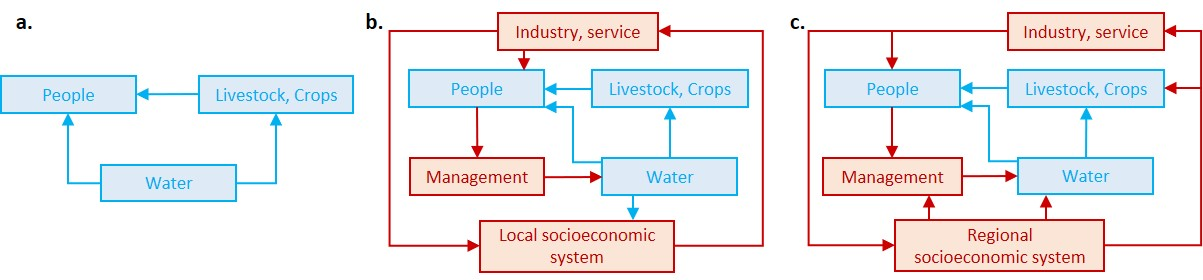
\includegraphics[width=0.9\textwidth]{main/framework.jpg}
	\caption{
		A framework for understanding the relationship between water governance regimes and transitions of a hydrosocial cycle. We aim to detect regime shifts using a simple and comprehensive index.
		% 图A是水资源利用的三个维度。每个维度都有两个极点(红色字表示),指示水资源利用在该轴上的两个变化方向。
		\textbf{A:} there are three key dimensions (supply, purpose and allocation) of water governance (see \textbf{Methods} for details). Each dimension has two poles (denoted in red) which indicate the two potential directions of changes along that axis: (1) ``supply'' shifts between scarcity and abundance. (2) ``purpose'' is weighted between consumptive services or non-consumptive uses. (3) ``allocation'' changes between balanced or lopsided.
		% 图B是将三个维度结合后的变化情况。因上述三个维度随着社会发展而不断变化,其组合的水资源利用状态也不同。这个过程中当突变发生时,可能标志着水资源利用发生了稳态转换,因此我们需要一个指标来监测其变化。
		\textbf{B:} along a trajectory of hydrosocial water cycle, governance changes are related to the combination of trends across the three dimensions. When abrupt change occurs, it may indicate a regime shift in water governance
		\cite{steffenTrajectoriesEarthSystem2018,abbottwatercycleAnthropocene2019,leviaHomogenizationterrestrialwater2020}.
	}
	\label{fig:framework}
\end{figure*}
